\chapter{Agent Theory}
\minitoc

Previously we mainly considered agent group perspective in which agents communicate, negotiate and coordinate their activities.\\
In this section, we will focus on individual perspective of agents, in the sense of how agents operate in terms of theoretical model architecture and mobility for implementing their particular task.\\
The first element of this individual perspective is called \side{Agent Theory}.

The reason why it is necessary to consider agent theory and formalisms is because formal theory has arguably had little impact on the general practice of software development, however, they are relevant in agent-based systems because we need to be able to give a semantic to the architecture, languages and tools that we use (i.e. a meaning).\\
Moreover without a semantic, it is never clear exactly what is happening and why it works.\\
But most importantly we need a theory to reach any kind of profound understanding the tools.

On the other hand the formalization of agents can be seen from 2 distinct perspective/purposes:
\begin{enumerate}
\item As \side{internal specification language} to be used by the agent in its reasoning or action
\item As \side{external metalanguage} to be used by the designer to specify, design and verify certain behavioural properties of agents situated in a dynamic environment.
\end{enumerate}

Agent theory gives us both an overview of the ways in which an agent is conceptualised and semantics to the architecture, language and tools: in other terms, we strive to formalise and conceptualise what is an autonomous entity and what is an autonomous behaviour.\\
Of course in order to have a theory of agent we need to introduce or consider a model of agents. For this purpose we will consider agents as\side{intentional systems}: the behaviour of an agent is explained in terms of attitudes such as believing and wanting.

\section{Agents as intentional systems}
Theorists start from the notion of an agent as an intentional system.\\
So, agent theorists start with the view of agents as intentional systems: where agent's behaviour is explained in terms of \side{attitudes}.
\subsection{Attitudes}
Attitudes represent a summary evaluation of a psycological object (e.g. oneself, other people, issue, plan, behaviour). We do not know for sure how it works, but it is our perception and psychological understanding.
For this reason attitudes are formed throughout the interaction with the surrounding environment and help to manage individual's cognitive resources to deal with uncertainties of complex dynamic domains.

In fact, the knowledge of the environment is seldom precise, agents may not know for sure or the environment may change. In this sense the agent knowledge is based on some uncertain element which prevents us to use plane knowledge base system as a foundation for agent. Moreover,  when dealing with autonomous entities we need a way to generate goals. And attitudes enable agents to express the knowledge about the world, as well as intentions and goals, similarly to humans.

Formally an attitude is the use of a folk psychology, by which human behaviour is predicted and explained through the attribution of attitudes.\\
Human however, do not act on attitudes, but rather use the notion of attitudes to explain their action. This is the reason why this formalism was chosen as a way to describe agent behaviour.

The attitudes employed in such folk psychological descriptions are called \side{intentional notions}.\\
An approach is to describe agent's behaviour in terms of intentional systems, ``whose behaviour can be predicted by the method of attrivutring belief, desire and rational acumen''.

An intentional system could be quite complex: first-order (attitudes), second-order (reasoning about attitudes),... etc.

Given all of the above, we might ask ourselver: is it useful to consider agents (similar to humans) as intentional systems? John McCarthy claims that:
\begin{itemize}
\item It is legitimate when it express the same information about the machine that it expresses about a person. 
\item It is useful when it helps us understand the structure of the artifact
\item It perhaps never logically required even for humans. \\
In fact, humans do not operate according to intentional notions but rather use attitudes and intentional notions to explain their action.
\item Ascription of mental qualities is most straightforward for machines of known structure but most useful for entities whose structure is incompletely known.\\
In simpler terms, if we completely know how a system works, then intentional systems are NOT useful. But the point is that agents do not and in fact cannot know exactly how the system works.\\
The more we know about a system the less we need to rely on intentional explanations of its behaviour.
\end{itemize}
An autonomous agent is a system that is most conveniently described by the intentional stance since it tries to mimic the behaviour of human which we do not know. 
\subsection{Theories of Attitudes}
We want to be able to design and build computer systems in terms of mentalistic notions.
Before we can do this, we need to identify a manageable subset of these attitudes and a model of how they interact to generate system behaviour. So first, which attitudes?

There exists 2 categories of attitudes:
\begin{enumerate}
\item \side{information attitudes}: which express the perception of the world (e.g. belief and knowledge)
\item \side{Pro-attitudes}: which guides agents behaviour (e.g. desire, intention, obligation, commitment, choice...)
\end{enumerate}
In principle, a good approach would be to choose at least one attitude from both of the categories.

The manipulation of these attitudes falls in the study of knowledge.
\subsection{Study of Knowledge}
The study of knowledge tries to answer a series of open questions:
\begin{itemize}
\item What do we know?
\item What can we know?
\item What does it mean to say someone knows something?
\item What does an agent need to know in order to perform an action?
\item How does an agent know whether it knows enough to perform an action?
\item At what point does an agent know enough to stop gathering information and make a decision?
\end{itemize}
In other terms, it is of our desire to formalise the intentional system in such a way that agent can reason about it.

Moreover, we need to distinguish between two different dimensions of knowledge:
\begin{itemize}
\item Individual perspective
\item Group perspective, which encompasses the knowledge of other agents in the group, \side{common knowledge} (e.g. traffic rules) and \side{distributed knowledge} (agents hold only a small portion of knowledge but only together can come up with the whole knowledge)
\end{itemize}


\section{Foundation of formal logic}

The formalisation of attitudes and knowledge requires some logical theory at its core.\\
A \side{formal logic} is a game for producing symbolic objects according to given rules. It can be interpreted as a sort of language with some general syntax or alphabet which include the following notation:
\begin{itemize}
\item Variables ($X,Y, ...$)
\item Constants ($a, abc, 15, ...$)
\item Functors ($f/n$) or functional symbol
\item Predicate symbols ($p,q,...$)
\item Logical connectivities ($\neg, \lor, \land, \rightarrow, \iff$)
\item Quantifiers ($\forall, \exists$)
\item Auxiliary symbols (commas, brackets and so on)
\end{itemize}

From this alphabet we can combine these elements to create words or \side{term}s ($T$):
\begin{itemize}
\item Any constant in $A$ is in $T$
\item any variable in $A$ is in $T$
\item if $f$ is an n-ary functor in $A$ and $t_1, ... , t_n \in T$ then $f(t_1,..., t_n) \in T$
\end{itemize}
Terms represent the basic building block of formal logic since they represents object to reason about, and as such they could be constant (constant term), variable (variable term) or structured object (functor).

Once we have defined what are the words or objects to discuss about, we can start to build up sentences as a set of terms or \side{formulae}.\\
Let $T$ be the set of terms over alphabet $A$ and $F$ is the set of formulae:
\begin{itemize}
\item If $p$ is an n-ary predicate symbol and $t_1,...,t_n \in T$ then $p(t_1,...,t_n) \in F$
\item If $H$ and $G \in F$ so are 
\[\neg{H} \quad H\lor G \quad H\land G \quad H \rightarrow G \quad H\iff G\]
\item If $H\in F$ and $X$ is a variable then $\forall X \in H$ and $\exists X \in F$ are formulae
\end{itemize}
Formulae of the form $p(t_1,..., t_n)$ are called \side{atomic formulae}.

\subsection{Interpretation}
Until now we considered the pure syntax and components of formal logic, the meaning or semantic in formal logic is given by the interpretation of an alphabet.\\
An interpretation $T$ of alphabet $A$ is a non-empty domain $D$ and a mapping that associates:
\begin{itemize}
\item $c \in Const$ with an element $c_t \in D [Const \subseteq A]$
\item $f/n \in Func$ with an element 
\[f_t: D_n \rightarrow D [Func\subseteq A]\]
\item $p/m \in Pred$ with an element 
\[p_T \subseteq D_m (= D\times ... \times D) [Pred\subseteq A]\]
\end{itemize}
In summary, both constant terms, functors (or structure object) and predicates (or relationship between objects) make up a domain.\\
The difference between predicate and functors is that predicate returns either true or false, the actual result of the predicate has to be deducted from the interpretation.\\
Under an interpretation, each term has a value and each atomic formula is either true or false.

We therefore defined the semantics of these objects or set of terms in the interpretation and equivalently we can formalize the semantics of the formulae or connectives of formal logic:
\begin{itemize}
\item \side{Negation}\\
$\neg{A}$ is true if $A$ is false
\item \side{Conjunction}\\
$A\land B$ is true if both $A$ and $B$ are true
\item \side{Disjunction}\\
$A\lor B$ is true if either $A$ or $B$ is true
\item \side{Implication}\\
$A\rightarrow B$ is true if either $\neg{A}$ or $B$ are true
\item \side{Universal quantifier} $\forall X$\\
$A(x)$ is true if $A$ is true for every $X$
\item \side{Existential quantifier} $\exists X$\\
$A(x)$ is true if $A$ is true for some $X$
\item \side{Propositional logic} is the logic of connectives (i.e. do not includes quantifier)
\item Adding quantifiers give first-order logic, sometimes called \side{predicate calculus}.
\item Adding quantifiers over formula variables give Higher Order Logic
\end{itemize}

We do not need classical formal logic to express something, we want to exploit this language to create a formalism that allow us to create new formulae from a given formula. There are two different ways to achieve this:
\begin{itemize}
\item \side{Models} and \side{Logical Consequence}\\
An interpretation $T$ is a model of a set of formulae $P$ iff every formulae of $P$ is true in $T$:
\begin{itemize}
\item every $P$ has infinitely many interpretations (because there exists infinite interpretation to the same symbol)
\item Not every $P$ has a model (e.g. $F \land \neg F$ cannot be true in the same interpretation)
\item A set of formulae is unsatisfiable if it has no model
\item A set of formulae is satisfiable if it has at least one model
\end{itemize}

Let $P$ be a set of formulae. $F$ is a logical consequence of $P$ ($P|=F$) iff $F$ is true in every model of $P$.\\
The symbol $|= $ indicates the logical consequence.

In some cases proving logical consequence is not necessary since, there already are some formulae that are equivalent in every intepretation. 
$F$ and $G$ are \side{logically equivalent} $(F \equiv G)$ iff $F$ and $G$ have the same truth value for every interpretation
\begin{align*}
F\rightarrow G &\equiv \neg F \lor G \\
F \rightarrow G &\equiv \neg G \rightarrow \neg F\\
\neg ( F\lor G) &\equiv \neg F \land \neg G\\
\neg ( F\land G) &\equiv \neg F \lor \neg G\\
\neg \forall X H(X) &\equiv \exists X \neg H(X)\\
\neg \exists X H(X) &\equiv \forall X \neg H(X)\\
...
\end{align*}
\item \side{Logical inference} does not consider the truth value but tries to process and manipulate a given set of formulae to create new ones.

Reasoning can be seen as a process of manipulation of formulae, which from a given set of formular, called \side{premises}, produces a new formula, called the conclusion using inference rules.\\
For instance \side{Modus Ponens}, states that if F is true and $F\rightarrow G$ then we can deduce that $G$ is true.

In simpler terms, we use a set of given formulae to deduce a new formula via inference rules.

Such deducability is represented with the notation:
$P\,\vdash \,F$ means F is derivable from P.\\
We can say that if the inference rules are sound then $P\vdash F$ (deducability) implies $P|=F$ (logical consequence)\\
If the inference rules are complete then  $P|=F$ (logical consequence) implies $P\vdash F$ (deducibility)

In other terms \side{soundness} states that everything that is deducible is true, whereas \side{completeness} says that everything that is true is deducible.
\end{itemize}

\section{Formalising attitudes}
Turns out that when we try to formalize attitudes or intentional systems, the application of formal logic makes them referentially opaque: hence standard substitution rules of first-order logic do not apply (intentional notions are not truth functional).
Hence in an interpretation the truth value of a formula depends on the truth value of each component, but in intentional systems belief can be true without proving the truth of what you believe.

We can conclude that this formalisation is not good enough for attributes. \\
There are 2 sorts of probelms to be addressed in developing a logical formalism for intentional notions:
\begin{enumerate}
\item Syntactic
\item Semantic
\end{enumerate}
With respect to the syntactic problem, there are two fundamental approaches:
\begin{enumerate}
\item Use a \side{modal language}, which contains modal operators, which are applied to formulae
\item use a \side{meta-language}: a first-order language containing terms that denote formulae of some other object language
\end{enumerate}
Likewise, two basic approaches to the semantic problem:
\begin{enumerate}
\item \side{Possible worlds semantics}
\item \side{Interpreted symbol structures}
\end{enumerate}
Of the four combination we will focus on the possible world semantics and modal logic


\subsection{Possible worlds}
The intuitive idea behind possible worlds is that besides the true states of affairs there are a number of states of affairs or ``worlds''.\\
Each world represents one state of affairs.\\
Given his current information, an agent may not be able to tell which of a number of possible worlds describes the actual state of affairs. Consequently, an agent's beliefs can be characterized as a set of possible worlds, which can be represented using modal logic.

The main advantages of such approach is:
\begin{itemize}
\item Mathematical theory is appealing
\item Neutral on the subject of the cognitive structure
\end{itemize}

Consider an agent playing a card game, who possessed the ace of spades. How could the agent deduce what cards were possessed by the opponents?\\
First, calculate all the various ways that the pack of cards could possibly have been distributed among the various players\\
Then, systematically eliminate all those configurations which are not possible given what the agent knows (any configuration in which the agent did not possess the ace of spades could be rejected).\\
Each configuration remaining after this is a world: a state of affairs considered possible given what the agent knows (aka \side{epistemic alternatives}).\\
We can notice that something true in all our agent's possibilities is known by the agent.

This approach/representation can be represented with a new form of logic known as \side{Modal logic}.
\subsection{Modal Logic}
Possible worlds can be incorpored into the semantic framework of modal logic.
In fact, modal logic was used by philosophers to investigate different \side{modes of truth} (e.g. possibly true and neceessarility true).

In the study of agents, it is used to give meaning to concepts such as belief and knowledge.\\
Modal logic can be considered as the logical theory of necessity and possibilty and it is essentially classical propositional logic extended by two operators:
\begin{itemize}
\item \side{Necessity } ($\square$)
\item \side{Possibility} ($\bDiamond$)
\end{itemize}
 
 And as a consequence, the syntax will be extended. Let $S=\{p,q,...\}$ be a set of atomic propositions
\begin{itemize}
\item If $p\in S$ then $p$ is a formula
\item If $A, B$ are formulae, then so are $\neg{A}$ and $A \land B$
\item if $A$ is a formulae, then so are $\square A$ and $\bDiamond A$
\end{itemize}
other connectives can be expressed by abbreviation:
\[F\rightarrow G \equiv \neg{F} \lor G q\qquad \neg{(F\land G)} \equiv \neg{F} \lor \neg{G}\]
This new operators can be expressed one from another, this is called duality of operators:
\[\square A \equiv \neg{\bDiamond} \neg{A}\qquad \bDiamond A \equiv \neg{\square} \neg{A}\]
In addition there are two basic properties that are true in this system:
\begin{enumerate}
\item \side{K axiom schema}
\[\square (A\rightarrow B ) \rightarrow (\square A \rightarrow \square B)\]
\item \side{Necessitation rule}: if A is valid, then $\square A$ is valid (A is true in all interpretation)
\end{enumerate}

The semantics of modal logic is traditionally given in terms of possible worlds:
\begin{itemize}
\item The formula $\square A$ is true if $A$ is true in every world accessible from the current world
\item The formula $\bDiamond A$ is true if $A$ is true in at least one world accessible from the current world
\end{itemize}
With sets of worlds as primitive, the structure of the model is captured by relating the different worlds via a binary accessibility relation.

Given all the above formalizing possible worlds via \side{Kripke structure}:
\[(S, \pi, K_1, ... , K_n\]
\begin{itemize}
\item $S$ is the set of possible worlds
\item $\pi$ is the set of formulae true at a world
\item $K_i$ is a binary accebility relation on $S$ (a set of pairs of elements of $S$)
\end{itemize}
\begin{figure}[!h]
\centering
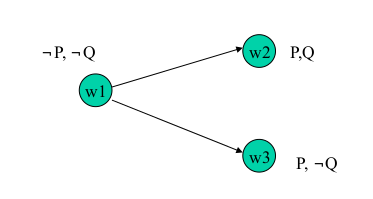
\includegraphics[width=.5\textwidth]{06/00}
\caption{Worlds $w_2$ and $w_3$ are accessible from world $w1$: modal logic states $\square P$ and $\bDiamond Q$. We can say nothing about world $w_1$ since it is not accessible/visible}
\end{figure}

This accessibility relation is given by a set of possible properties related to the worlds:
\begin{itemize}
\item \side{Reflexive} (a world can see itself)\\
For all $s\in S$, we have $(s,s)\in K$
\item \side{Symmetric} (two worlds are mutually accessible)\\
For all $s,t \in S$, we have $(s,t)\in K \iff (t,s)\in K$
\item \side{Transitive}\\
For all $s,t,u \in S$, we have that if 
\[(s,t)\in K \qquad \land (t,u)\in K \quad\text{then}\quad (s,u)\in K\]
\item \side{Serial} (a world can access at least another world)\\
For all $s\in S$ there is some $t$ such that $(s,t)\in K$
\item \side{Euclidean}\\
For all $s,t,u\in S$ whenever
\[(s,t)\in K \quad\land\quad (s,u)\in K\quad\text{then}\quad (t,u)\in K\]
\end{itemize}
From the above we deduce that:\\
If $K$ is Reflexive and Euclidean, then $K$ is symmetric and transitive\\
If $K$ is Symmetric and transitive, then $K$ is Euclidean

The following are equivalent:
\begin{itemize}
\item K is reflexive, simmetric and transitive
\item K is symmetric, transitive and serial 
\item K is reflexive and Euclidean
\end{itemize}
Hence we determine which world are accessible by analysing the properties of the relations between such worlds.

Properties of accessibility relation can be expressed by axiom schemas:
\begin{itemize}
\item \side{T axiom}: corresponds to reflexive accessibility relation
\[\square A \rightarrow A\]
\item \side{D axiom}: corresponds to serial accessibility relation
\[\square A \rightarrow \bDiamond A\]
\item \side{4 axiom}: corresponds to transitive accessibility relation
\[\square A \rightarrow \square\square A\]
\item \side{5 axiom}: corresponds to Euclidean accessibility relation
\[\bDiamond A\rightarrow ]square \bDiamond A\]
\end{itemize}

Depending on which axiom we include in our logic we can derive different types of logic which are referenced with the notations:
\[S5(KT5)\qquad S4(KT4)\qquad T(KT) \qquad weak-S5(KD45)\]
This is important since for belief and knowledge logic there will be different sets of axioms.

\section{Logic of Knowledge}
Finally, we have all the tools to formalise knowledge, and this will be done by changing the meaning or interpretation of the symbols, not the axiom of the modal logic.

The formula $\square A$ is read ``It is known that A'' of ``agent knows A'' and denoted as $K$\\
For group knowledge we have an indexed set of modal operators:
\[K_1, ...., K_n \quad\text{for }\square\]
In this frame of reference $K_1 A$ is read as ``agent1 knows A''

As a consequence, we can interpret the 4 axiom of accessibility relation:
\begin{itemize}
\item T axiom (Knowledge axiom) $K_i A \rightarrow A$\\
\say{what is known is true}
\item D axiom $K_i A \rightarrow \neg{K_i} \neg{A}$\\
\say{If agent i knows A then agent i does not know $\neg{A}$}
\item 4 axiom (positive introspection) $K_i A \rightarrow K_i K_i A$\\
\say{If agent i knows A then agents i knows that it knows A}
\item 5 axiom (negative introspection) $\neg{K_i} \neg{A}\rightarrow K_i \neg{K_i}\neg{A}$\\
\say{agent i is aware of what it does not know} 
\end{itemize}

Knowledge is often defined as true belief, i.e. an agent knows A if the agent believs A and A is true.\\
Axioms KTD45 are often chosen as a logic of knowledge.\\
Axioms KD45 are often chosen as a logic of belief (T does not hold since what is believed is not necessarily true).\\

How well does normal modal logic serves as a logic of knowledge and belief? There are two main problems related to the K axiom and the necessitation rule. In fact, the interpretation changes from the logic of belief and the logic of knowledge 
\begin{itemize}
\item Necessitation rule: an agent knows all valid formulae (an agent will have an infinite number of items of knowledge)\\
If $A$ is valid, then $\square A$ is valid
\item K axiom: agent's knowledge is closed under implication
\[\square(A\rightarrow B) \rightarrow (\square A \rightarrow \square B)\]
\end{itemize}
This leads to the logical \side{Logical omniscience problem}: constituted by that of knowing all valid formulae and that of knowledge/belief being closed under consequence (must know all logical consequences of one's knowledge or belief).

This means that in this system logic, agents believe/know all valid formulae and agents' beliefs/knowledge are closed under logical consequence.

Other approaches that were propesed to avoid the logical omniscence problem are:
\begin{enumerate}
\item \side{Levesque}\\
In order to avoid logical omniscience problem a distinctrion is made between explicit (what the agent knows by experience and perception) and implicit belief (what the agent deduce from what is known).
\item \side{Konolige}\\
Deduction model of belief\\
The deduction model defines a belief system as a tuple
\[d=(\Delta, \rho)\]
containing a base set of formulae in some internal, logical language of belief and a set of deduction rules (may be incomplete) for deriving new beliefs\\
Agent with such a belief system believe $A$ if $A$ can be derived from its base set using its deduction rules
\end{enumerate}


\section{BDI architecture}
We have all the tools to apply this logic and consider the combinations of a small set of attitudes and see how they can be expressed in formal theory.\\
Systems and formalisms that give primary importance to intentions are often referred to as \side{BDI architecture}.\\
Formalization of intentions based on branching-time possible worlds future and single past model.\\

In addition to possible worlds semantics Rao and Georgeff, decided to consider what happens inside a single world and they find out the relations of what happens in one world between different attitudes


Crucial elements are :
\begin{itemize}
\item Intentions are treated on a pair with beliefs and goals
\item Distinguishes between choices and the possibilities of the different outcomes of actions
\item Interrelationship between belief, goals and intentions are specified (goals are consisten desires of an agent)
\end{itemize}

They formulated some informal semantics:
\begin{itemize}
\item The world is modeled by using a temporal structure with a branching time future and a single past, this is called a \side{time tree}
\item A particular time point in a particular world is a \side{situation}
\item Event types transform one time point to another
\item Primitive events are those events directly performable by the agent and uniquely determine the next time point
\item The brances in a time tree represent the choices available to an agent
\end{itemize}
To model this informal semantics they chose to use 2 modal operators:
\begin{itemize}
\item \side{Optional}: a path formula (path along a time tree) is said to be optional if, at a particular time point in a time tree, it is true of at least one path emanating from the point
\item \side{Inevitable}: a path formula is said to be inevitable if it true of all paths emanating from that point
\end{itemize}
In addition, they provided some additional \side{Temporal operators}: next, eventually (appears at the end of a path in time tree), always (appears in every node of a path) and until.\\
A combination of these modalities can be used to describe the options available to an agent.\\

BDI Architecture states that there are three basic attitudes:
\begin{enumerate}
\item \side{Beliefs}\\
In each situtation a set of belief-accessible worlds is associate. Those worlds that the agent believes to be possible.\\
Each belief-accessible world is a time-tree
\item \side{Goals/Desires}\\
For each situation a set of goal-accessible worlds is associated. Those represent the goals of the agent.\\
Goals are chosen desires of the agent that are consistent and agent should believe that the goal is achievable; goals must be compatible with beliefs.\\
For each belief-accessible world w in time t, there must be a goal accessible sub-worlds of w at time t.

In particular goals are desires that we believe to be achievable.\\
In each world, there is a time tree that can be structured as a belief structure. Goals/desires are substructure of such structure  because we choose only the paths/goals that we believe achievable (scuh substructure is called goal tree).
\item \side{Intentions}\\
Intentions are represented by a set of intention-accessible worlds\\
These worlds are ones that an agent has committed to attempt to realize\\
The intention-accessible worlds of an agent must be compatible with its goal-accessible worlds\\
For each goal-accessible world w in time t, there must be an intention accessible sub world of w at time t
\end{enumerate}

An agent perceivs the world and understand what is believable.
From what is believable some of these points can be chosen as goals. And from this we can choose some goals (intentions) to which we commit to execute.